\chapter{Proposed methodology}\label{methodology}

\lettrine{T}{unable} applications are characterized by the presence of specific parameters, also known as \textit{knobs}, that influence program execution; their change produces different application results in terms of metric of interest values, as, for instance, throughput or power consumption. Figure \ref{fig::appDef} shows a typical parallel architecture with three nodes (node 1, 2 and 3) that are executing three tunable applications (application X, Y and Z respectively):

\begin{figure}[H]

    \centering
    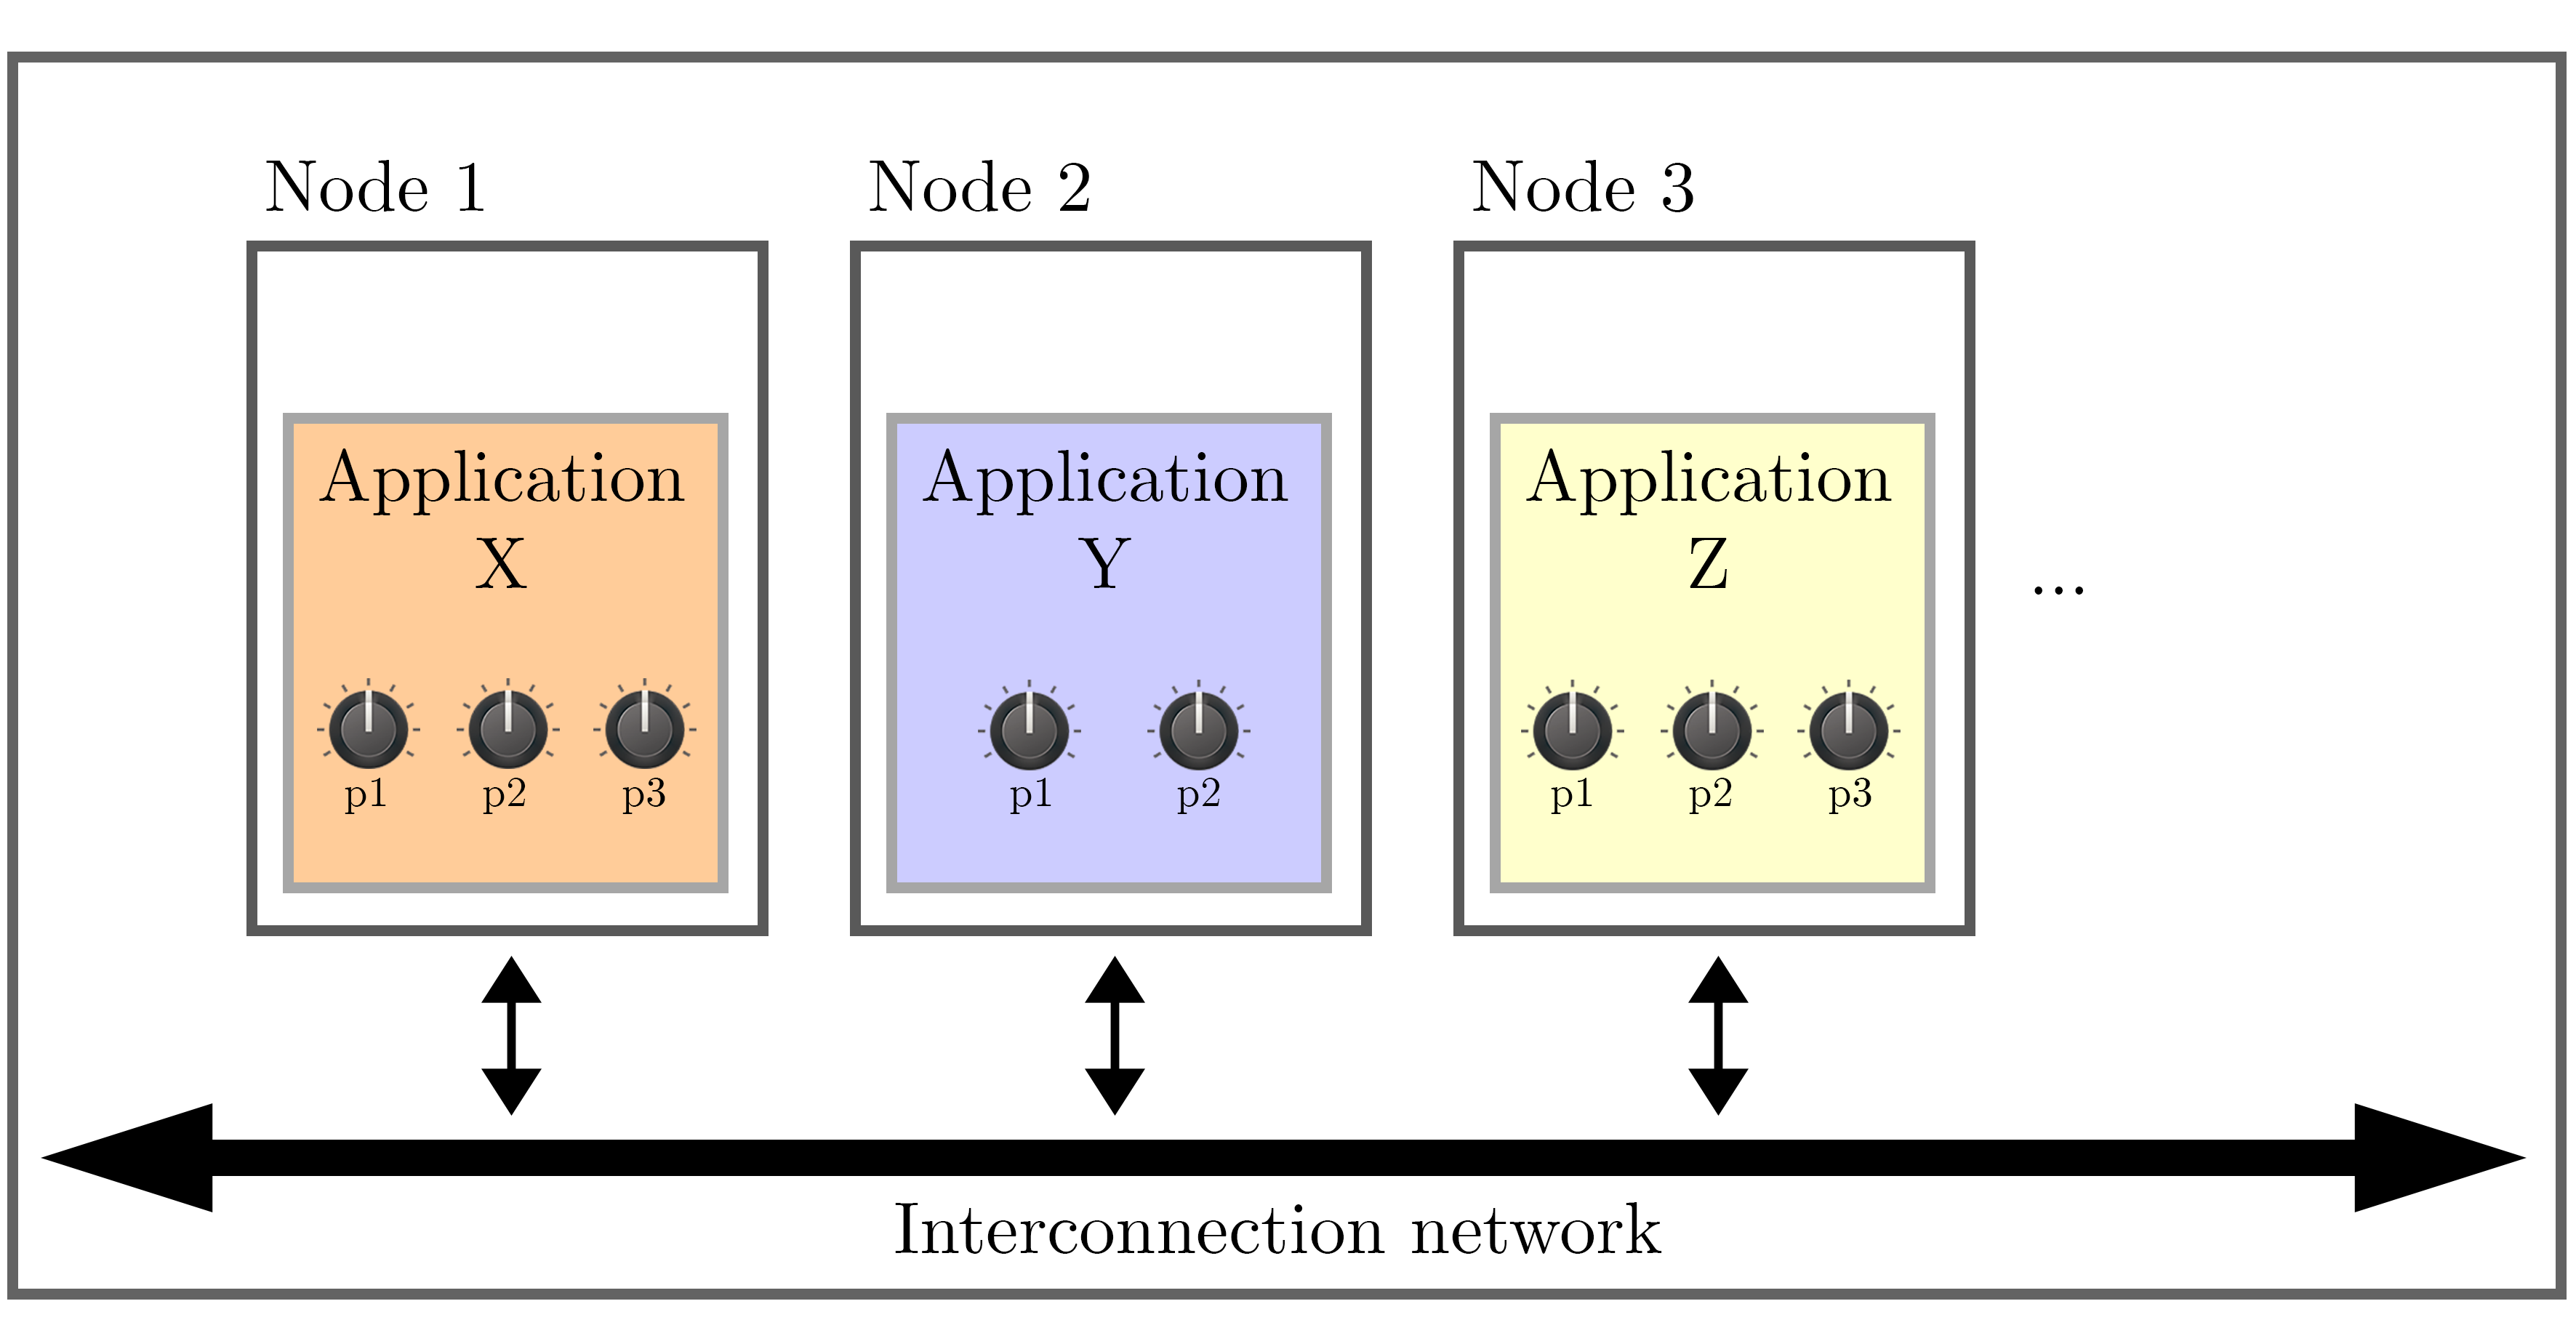
\includegraphics[width = \textwidth]{Apps}
    \caption{An example of a parallel architecture with three executing tunable applications; application X on node 1 and application Z on node 3 have three knobs, application Y on node 2 two ones}
    \label{fig::appDef}
    
\end{figure}

Very often, High Performance Computing applications expose a large set of parameters, making related Design Space huge and, consequently, unrealistic to explore it in an exhaustive way; in order to choose, from time to time, best program setting with the aim to improve energy efficiency with respect to power consumption and current input data, the concept of runtime autotuning is used: a class of online autotuners is able to choose, from time to time, best possible parameter values that fulfill application goals and requirements, starting from a design-time knowledge that gives information about parameter values and corresponding metric of interest values, built off-line. Figure \ref{fig::appAut} shows application Z interconnected with mARGOt \cite{gadioli2015application}, a dynamic autotuner developed by our research group:

\begin{figure}[H]

    \centering
    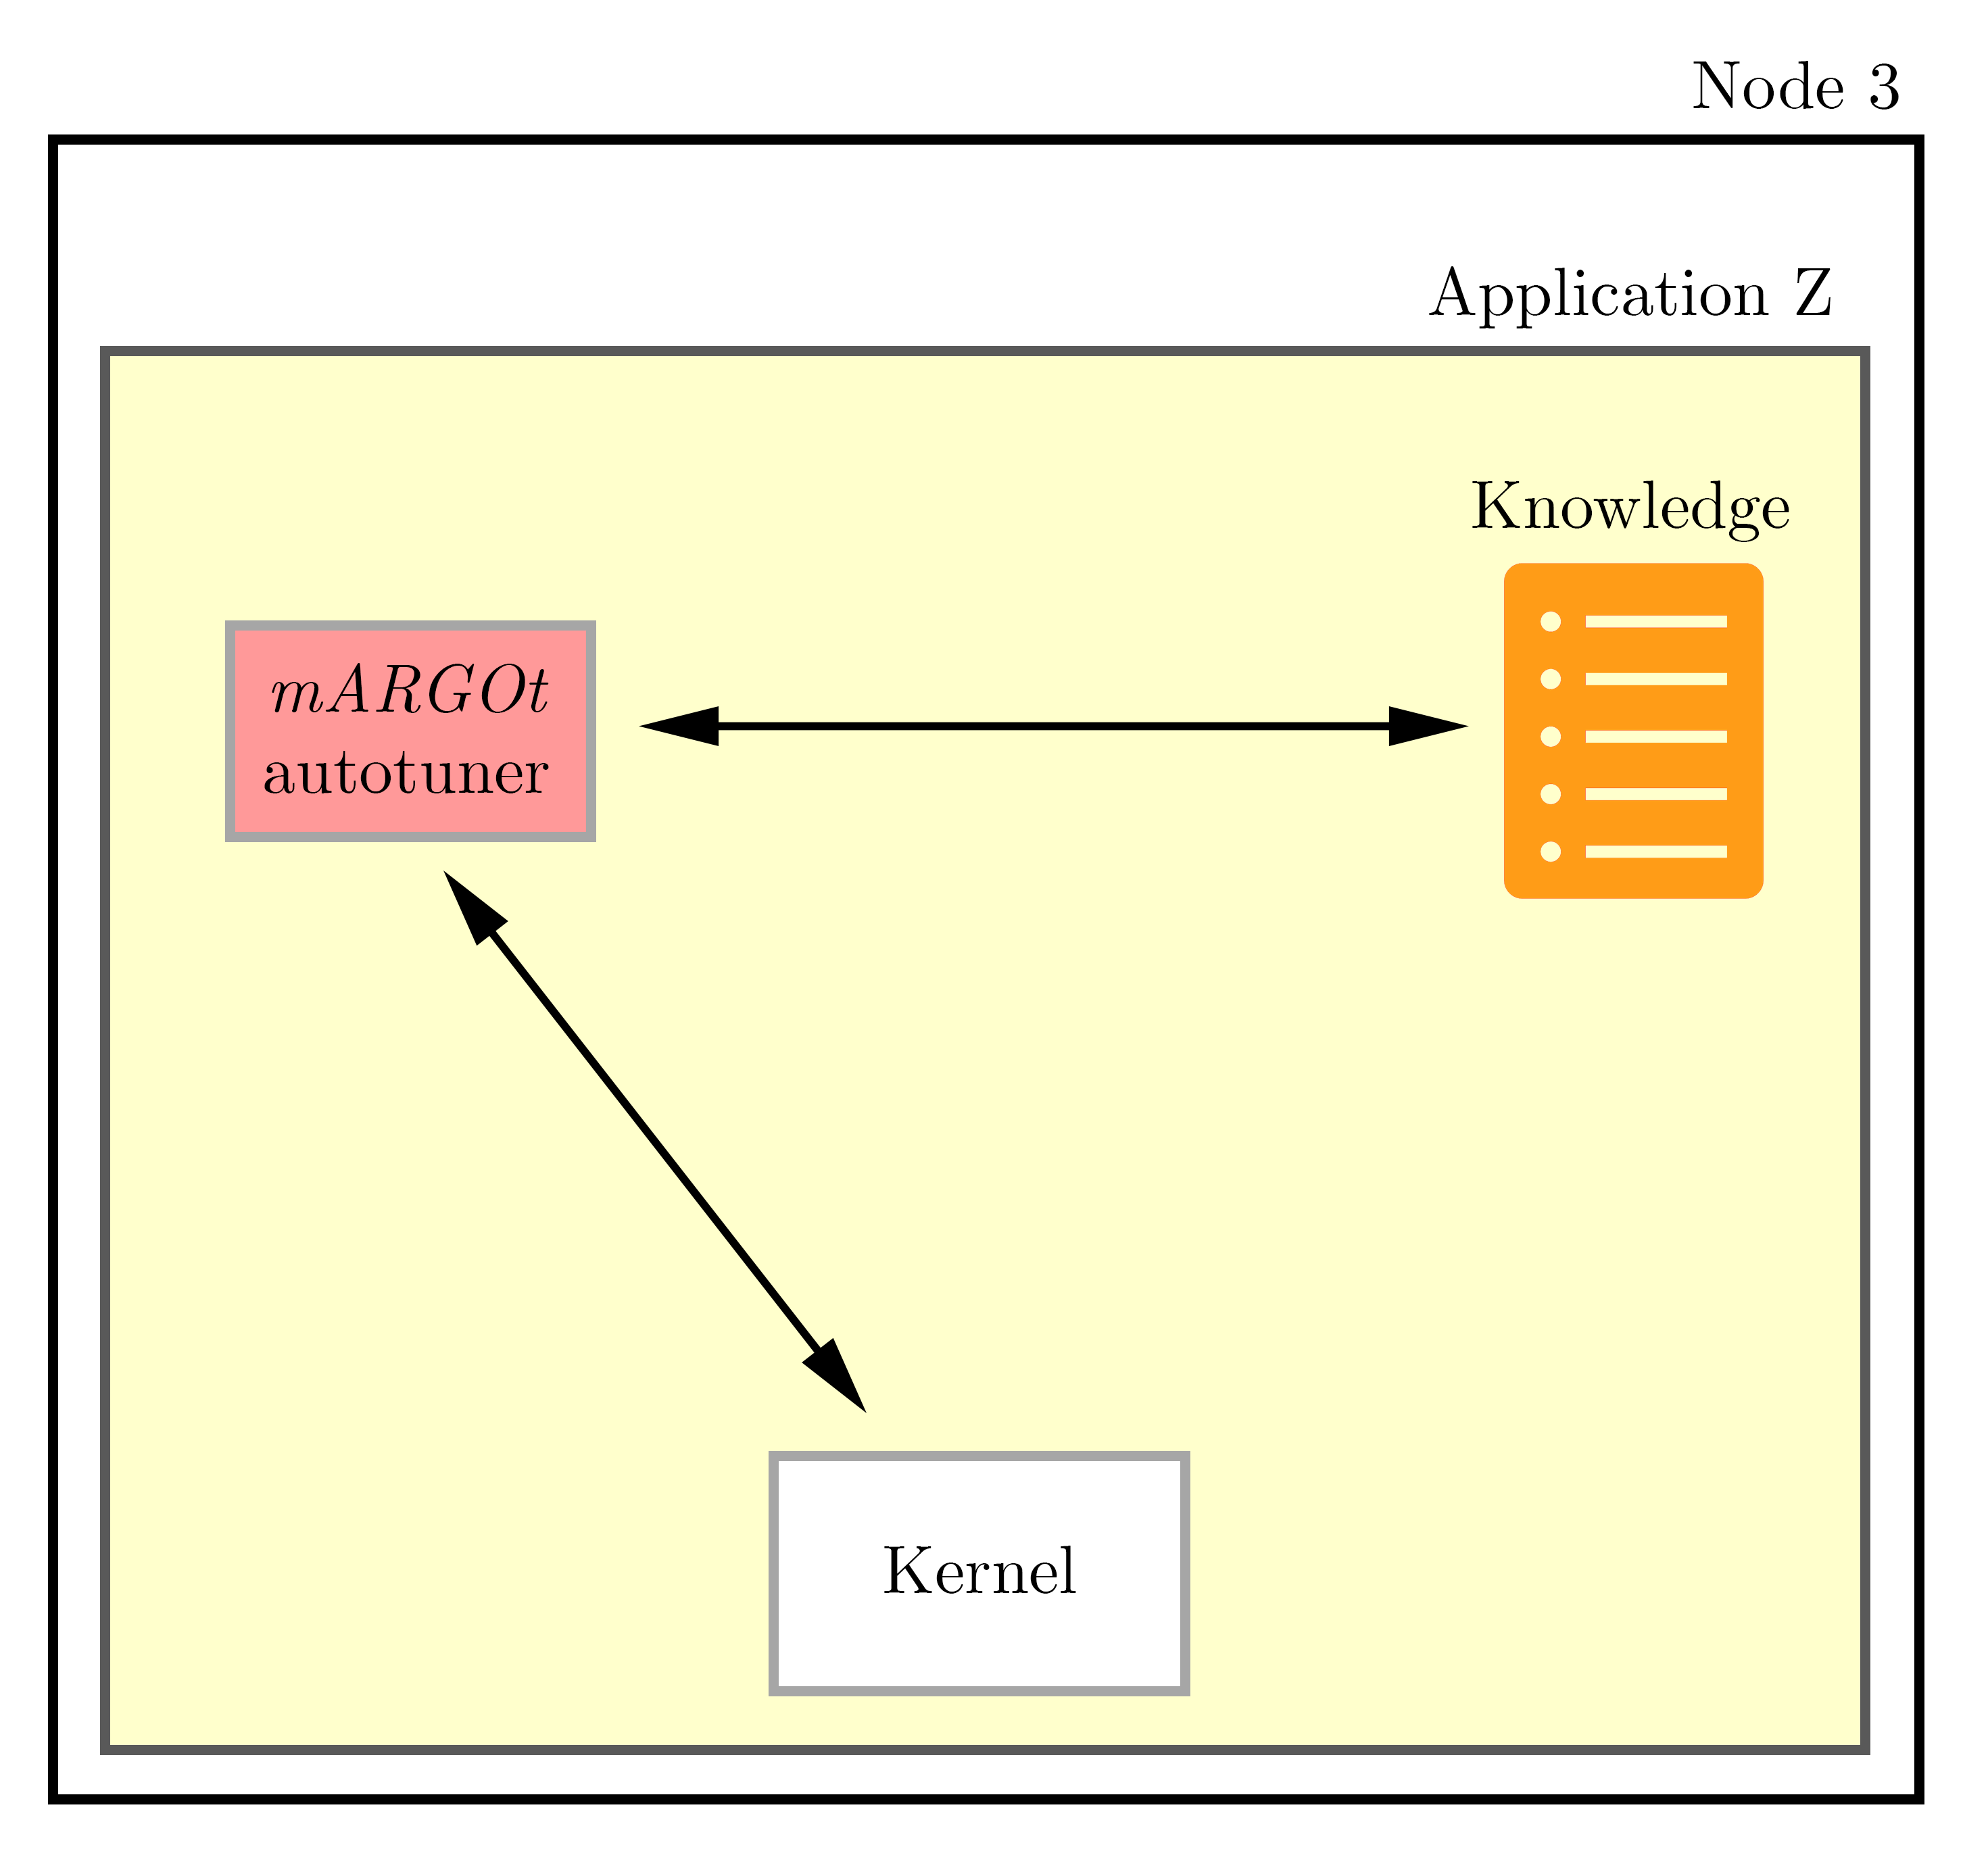
\includegraphics[width = \textwidth]{App_mARGOt}
    \caption{Tunable application Z with the assistance of mARGOt autotuner schema}
    \label{fig::appAut}
    
\end{figure}

As we can understand, this kind of autotuner needs application knowledge, so there have to be a preceding phase, before program start of computation, in which it is made; our improvement is to avoid this offline step, building, managing and updating application knowledge during execution itself. A local module mainly takes care of properly setting application knowledge, while a remote one manages collected information during execution, in order to predict complete application model. Figure \ref{fig::appAGORA} shows application Z interconnected with Agorà plus mARGOt autotuner:

\begin{figure}[H]

    \centering
    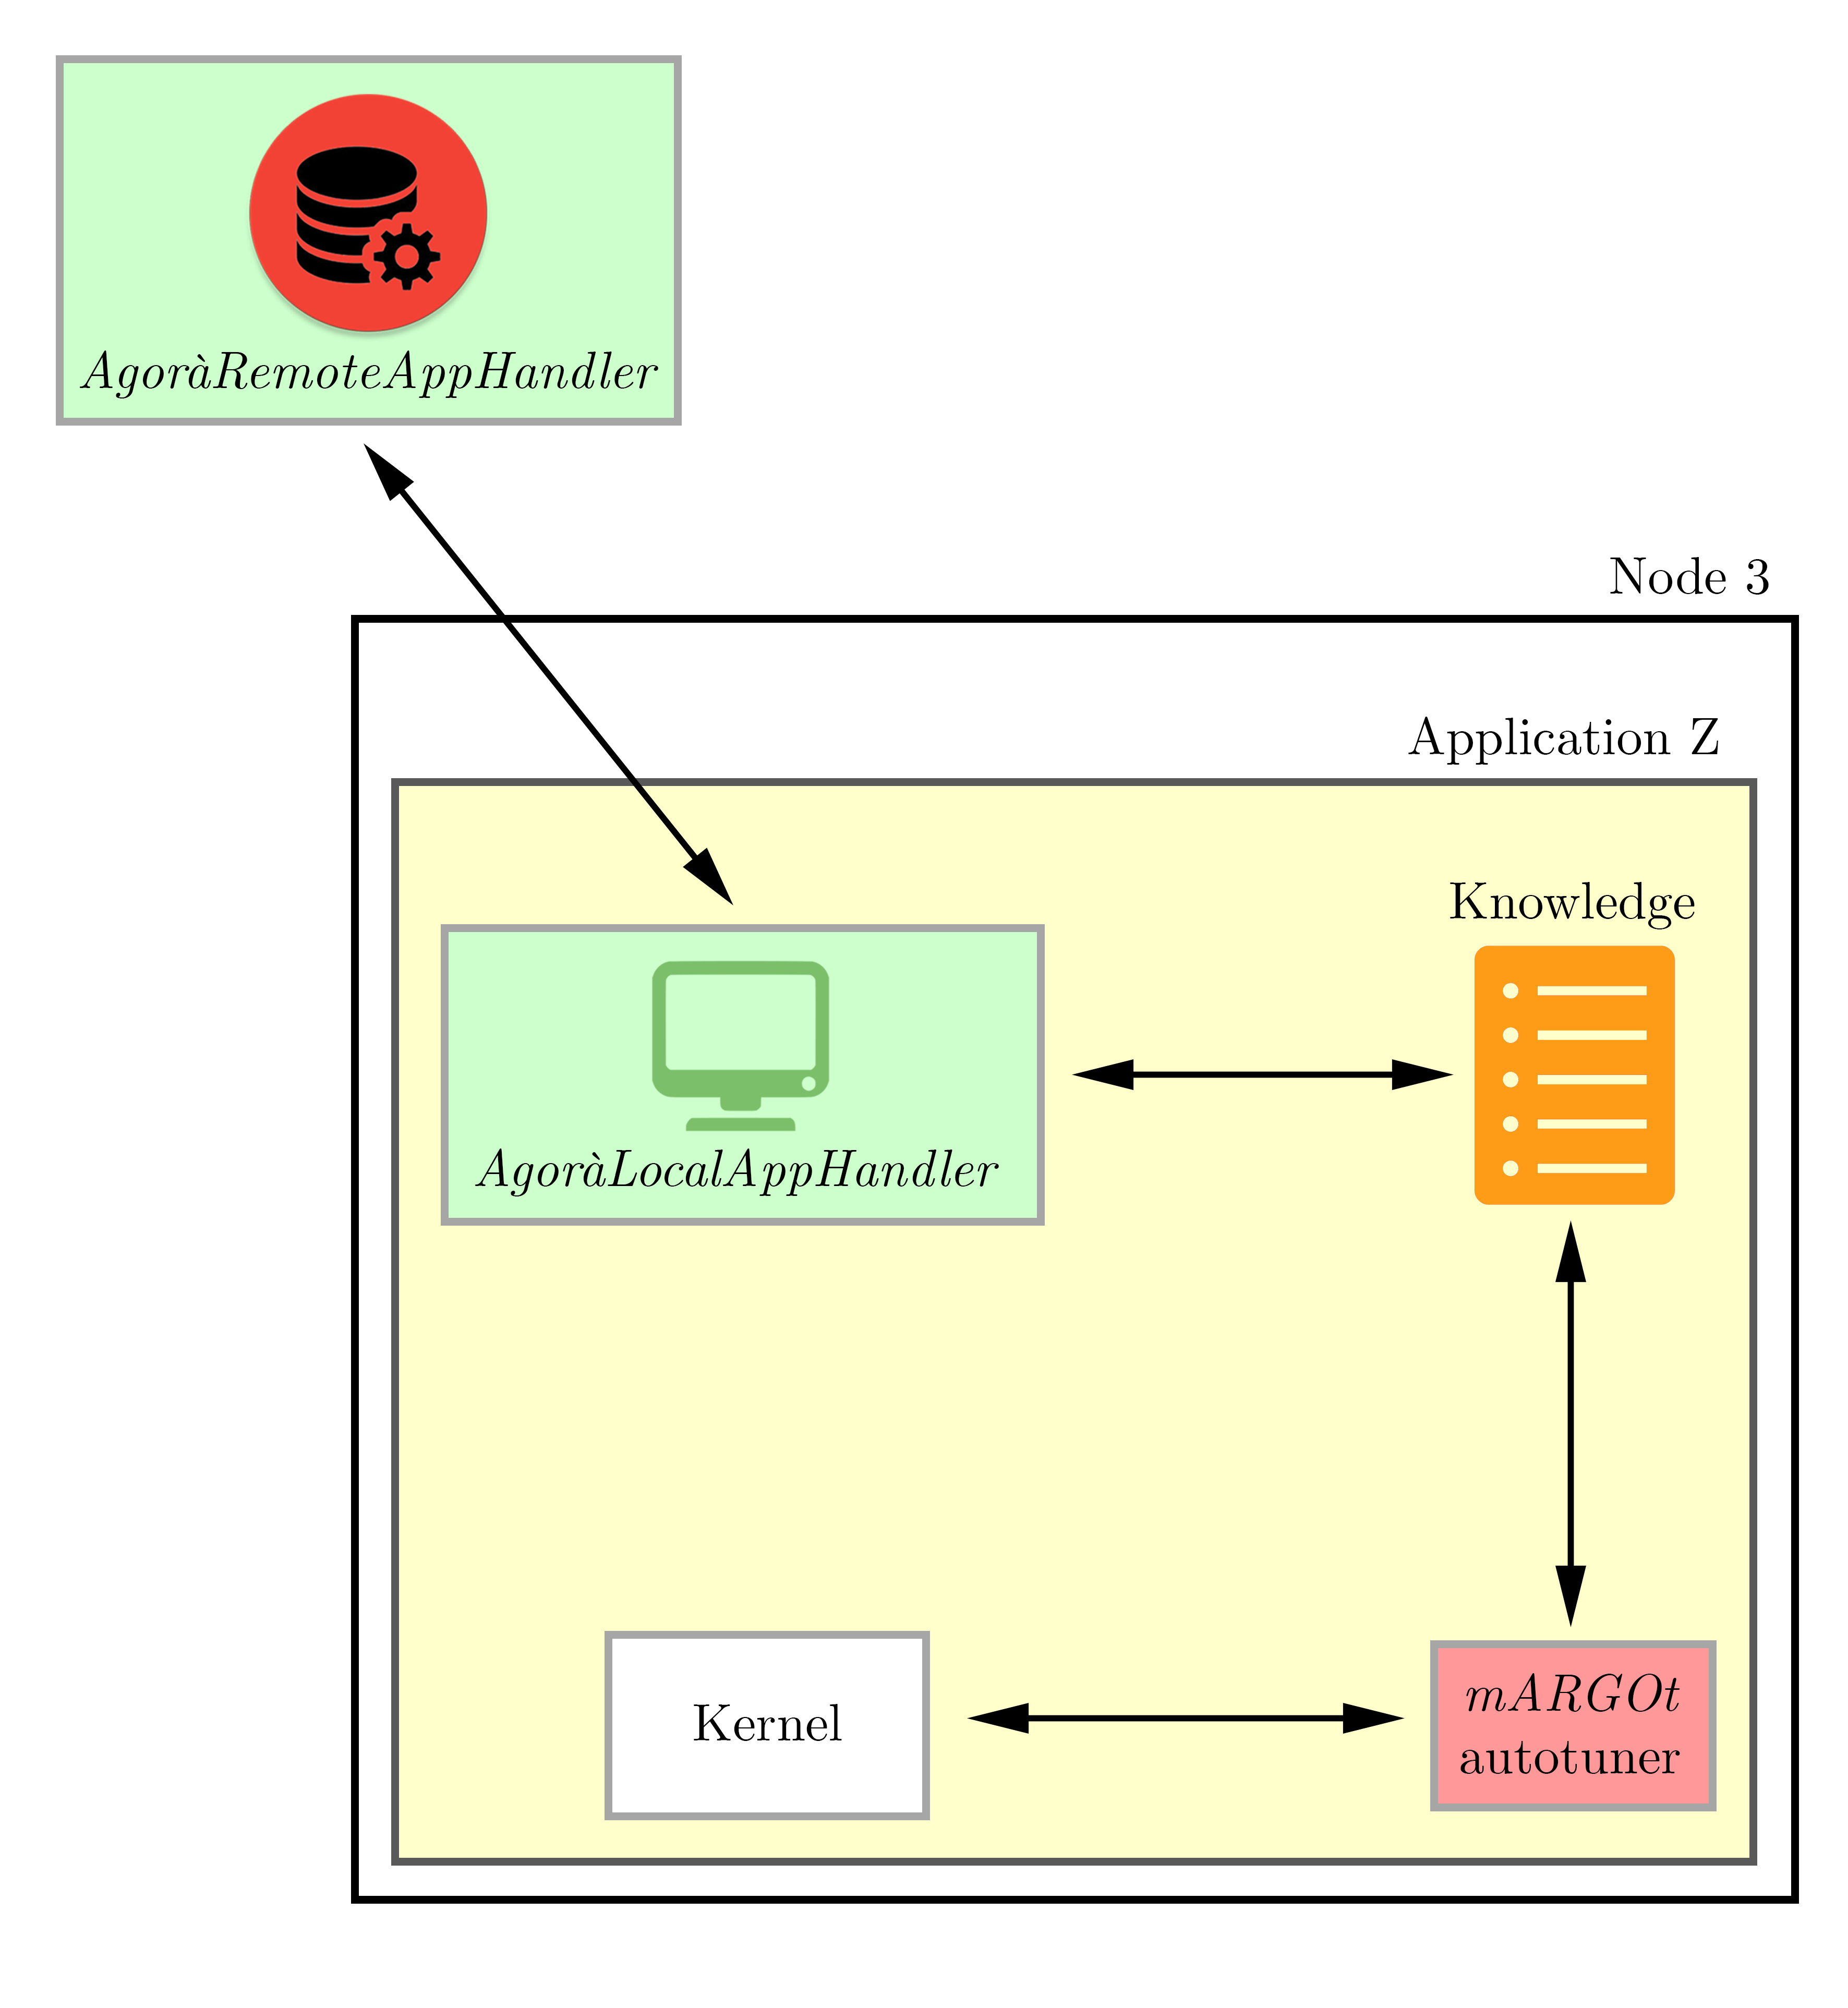
\includegraphics[width = \textwidth]{App_Agora_mARGOt}
    \caption{Tunable application Z with the assistance of Agorà plus mARGOt autotuner schema}
    \label{fig::appAGORA}
    
\end{figure}

This work, therefore, wants to address the problem of managing possible multiple applications that run, at the same time, inside a parallel architecture; main objective is to initially drive program execution with a subset of parameter configurations taken from their Design Space, in order to gather all metric of interest values associated to them; this list composes the training set for the prediction of application complete model through Machine Learning techniques. Agorà can also correctly manage possible features; a feature is a particular application element than can not be set up like software knobs, but it contributes to the estimation of complete model; during DSE phase, feature values are observed like metric values while, during model prediction, they are considered as parameters, so their observations take part to the estimation of metric of interest values.

The typical architecture in which Agorà works is a parallel one, where there are multiple nodes, potentially heterogeneous, that execute applications; principal Agorà strenghts are:

\begin{enumerate}
    
    \item the ability to drive Design Space Exploration in a distributed way, among all nodes that are running the same program, in order to considerably reduce DSE phase and to speed up overall workflow;
    
    \item the ability to manage multiple kinds of applications, each of them separately organized by a dedicated Agorà module that is in charge of all nodes that execute the same program;
    
    \item the out-of-band activity from parallel architecture data streams: computation of Design of Experiments configurations, collection of associated metric of interest values and complete model prediction are done in a separate node with respect to the ones that run applications inside the architecture, while the exchange of information is done using the lightweight MQTT protocol (discussed in chapter \ref{mqtt});
    
    \item the persistence of generated knowledge: once application complete model is predicted, it is stored so, at any time, it can be reloaded and it is sent to new nodes that start running the same application, without repeating all the workflow through which the complete model has been previously predicted;
    
    \item the capability of being fault-tolerant, with respect both to a running node crash and to the interruption of remote Agorà module that has the objective to predict application complete model: if the former situation happens, Agorà has to properly handle remaining running nodes; if the latter situation happens, running nodes inside the parallel architecture does not have to stop their execution but they react properly, according to the internal state of their related local Agorà module at that moment.

\end{enumerate}

\begin{figure}[H]

    \centering
    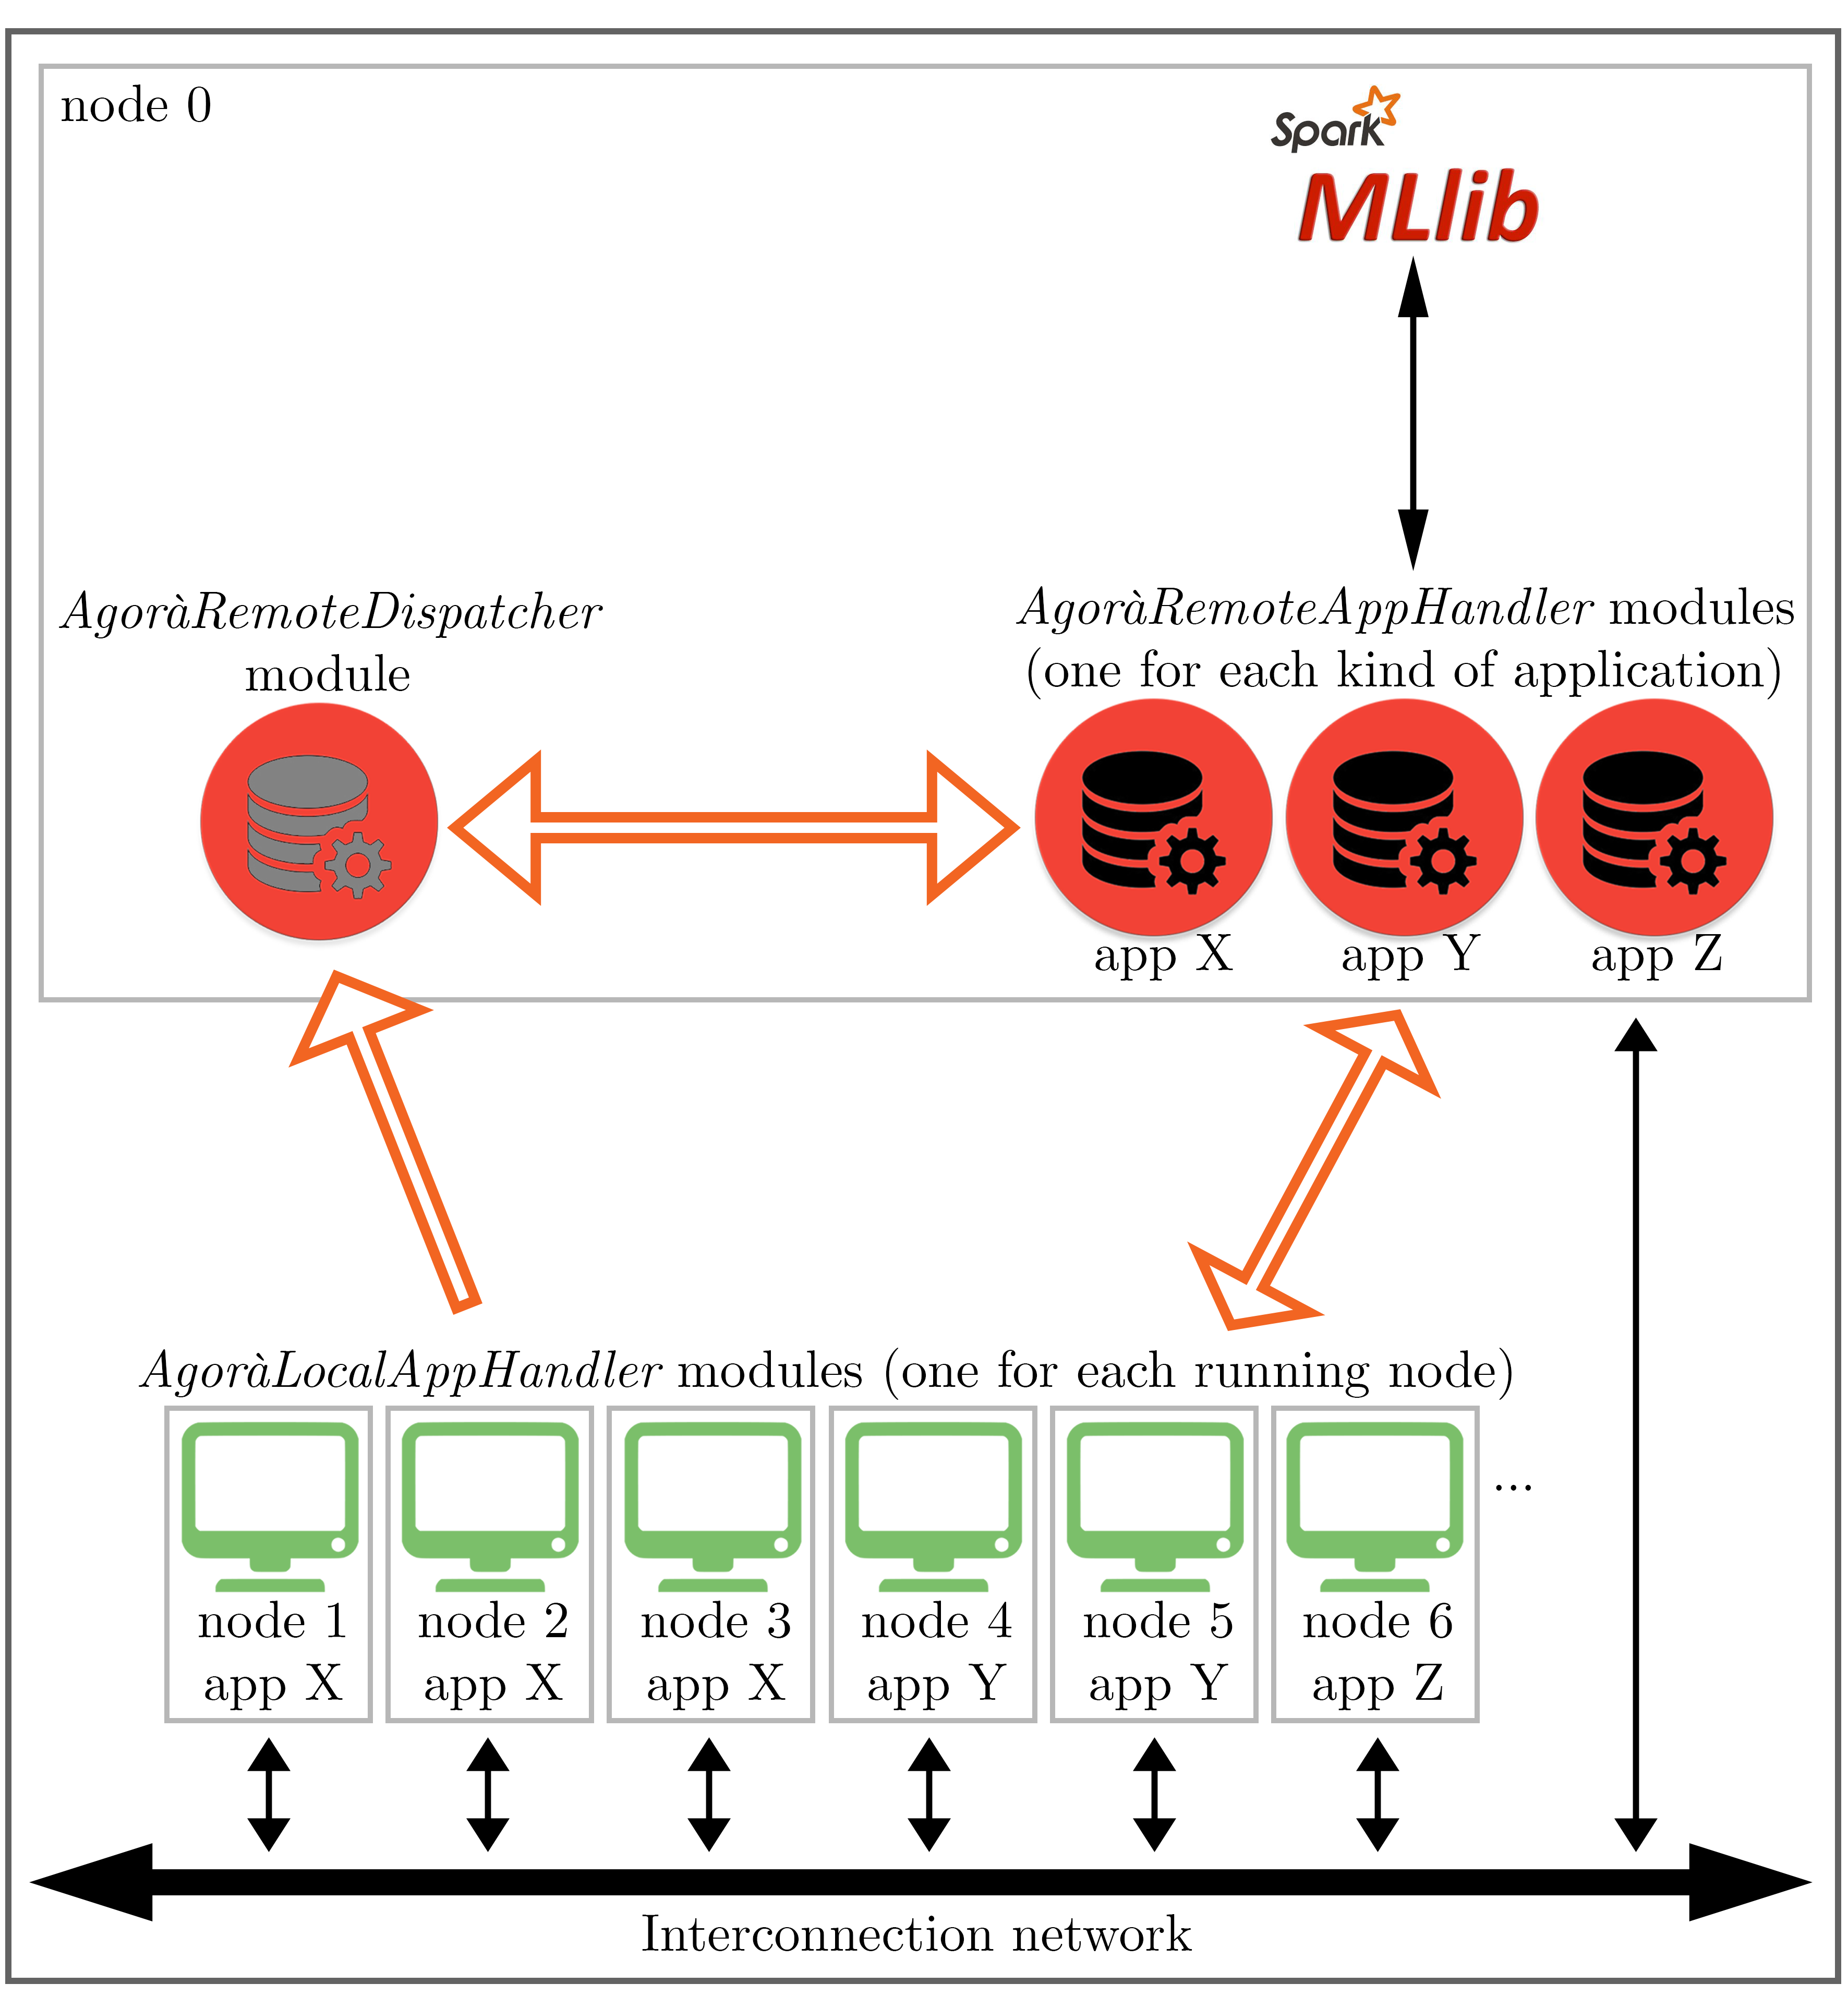
\includegraphics[width = \textwidth]{Agora_overall}
    \caption{Agorà overview in a parallel architecture}
    \label{fig::tesiCris_overview}
    
\end{figure}

Figure \ref{fig::tesiCris_overview} shows all Agorà components and a possible scenario with a parallel architecture in which six nodes are running three different tunable applications; for every kind of application there exists a dedicated AgoràRemoteAppHandler module that manages it; orange empty arrows represent all possible communications among modules, made possible through MQTT subscriptions and publications on predetermined topics.

Agorà main components are:

\begin{itemize}

    \item the \textit{AgoràDispatcher} module, written in Python: it keeps waiting for program arrival, in order to properly manage them;
    
    \item the \textit{AgoràRemoteAppHandler} module, written in Python: it is created by the AgoràDispatcher for every kind of application; it asks for application information such as, for instance, all parameter name and values; it computes application configurations that compose the Design of Experiments; it drives Design Space Exploration phase, distributing DoE configurations among all nodes it manages; it collects parameter values and the observed metrics of interest sent by running programs; it makes use of Machine Learning techniques in order to build application complete model; it sends result to connected nodes;
    
    \item the \textit{AgoràLocalAppHandler} module, written in C++: it is set up in every executing program; it communicates with the autotuner that manages application behavior; it notifies the existence of related running machine to the AgoràDispatcher module; it replies to possible information request made by the related AgoràRemoteAppHandler; during Design Space Exploration phase, it receives configurations from the AgoràRemoteAppHandler module, it sets up program knowledge with this information and, after the application has done computation, it sends back all obtained information, regarding parameter values and associated metric of interest values; it saves predicted complete model received from the AgoràRemoteAppHandler module, in order to properly update application knowledge with this data.

\end{itemize}

Principal use cases that define framework workflow and the interaction among components are the following:

\begin{enumerate}

    \item application start of execution: when programs start running, related AgoràLocalAppHandler module notifies their existence to the AgoràDispatcher module; if the application is unknown, AgoràDispatcher creates a dedicated AgoràRemoteAppHandler module that is in charge of managing it, otherwise it communicates new node to the corresponding existing AgoràRemoteAppHandler module;
    
    \item Design of Experiments computation: AgoràRemoteAppHandler module computes the subset of configurations, from the entire application Design Space, that compose the Design of Experiments; after that, it is ready to drive Design Space Exploration phase, distributing these configurations to requesting nodes;
    
    \item configuration reception: AgoràLocalAppHandler module updates application knowledge with all the configurations that, from time to time, are sent by the AgoràRemoteAppHandler module; every time program computation is finished, it sends back to the AgoràRemoteAppHandler module a list of values, made by the configuration just used with the observed metrics of interest;
    
    \item application configuration and related metric value collection: A\-go\-rà\-Remote\-App\-Handler module collects all the information it receives from running nodes; when it has all necessary data, it uses Machine Learning techniques in order to predict application complete model, made by all possible configurations associated with predicted metric values;
    
    \item predicted model dispatch: application complete model is sent by AgoràRemoteAppHandler to associated running nodes; related AgoràLocalAppHandler modules update program knowledge with this information, so the dynamic autotuner can set up application knobs with the best configuration that fulfills current goals and requirements.

\end{enumerate}

The interaction among Agorà components is implemented in an asynchronous way: program executions are independent from MQTT message exchange and all modules properly react to these events, in order to not condition application workflow and to not steal execution time, making all process as flowing as possible.
